\documentclass[11pt]{article}
\title{\textbf{Meccano nonagon}}
\author{https://github.com/heptagons/meccano/nona}
\date{}

\usepackage{../meccano}

%\usepackage{amsmath}
%\usepackage[pdftex]{graphicx}

\begin{document}

\maketitle

\begin{figure}[h]
\centering
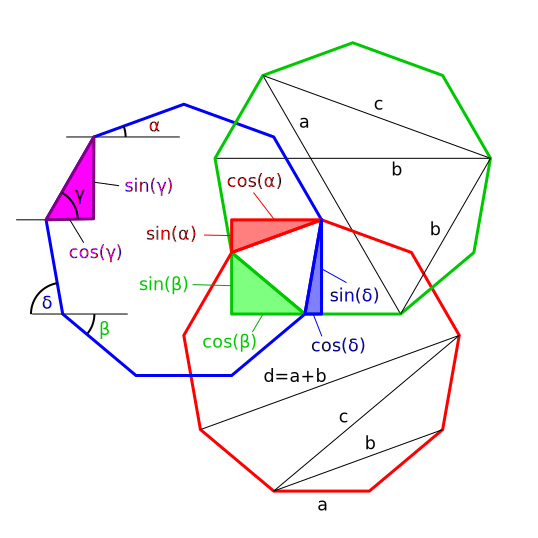
\includegraphics[scale=0.7]{figs/3nonagons}
\caption{Three regular nonagons connected by an equilateral triangle.
We note four angles in the figure $A$, $B$, $C$ and $D$.}
\label{fig:nonagons}
\end{figure}





\section{Algebra}

Figure \ref{fig:nonagons} shows three regular nonagons connected by an equilateral 
triangle. Four angles appear orthogonally in any regular nonagon:
\begin{align}
\alpha &= \pi/9 = 20^{\circ} \\
\beta &= 2\pi/9 = 40^{\circ} \\
\gamma &= 3\pi/9 = 60^{\circ} \\
\delta &= 4\pi/9 = 80^{\circ} \\
\alpha + \beta &= \delta - \alpha = \gamma
\end{align}

The relations of angle $C$ are those of equilateral triangle:
\begin{align}
\cos\gamma &= -\frac{1}{2}\\
\sin\gamma &= \frac{\sqrt{3}}{2}
\end{align}

From the figure \ref{fig:nonagons}, cosines of angles $\alpha, \beta, \delta$ are related as:
\begin{align}
\cos\alpha &= \cos\beta + \cos\delta \label{eq:cosines-alpha-beta-delta-sum} \\
 &= \cos(2\alpha) + \cos(4\alpha) \nonumber\\
 &= (2\cos^2\alpha - 1) + (1 -8\cos^2\alpha + 8\cos^4\alpha) \nonumber\\
 &= 8\cos^4\alpha - 6\cos^2\alpha \nonumber\\
 1 &= 8\cos^3\alpha - 6\cos\alpha
\end{align}

Previous cosines equation is the depressed cubic equation with a negative discriminant:
\begin{align}
t^3 +pt +q &= 0 \label{eq:cubic}\\
p &= -\frac{3}{4}\\
q &= -\frac{1}{8}\\
\Delta &= \frac{q^2}{4} + \frac{p^3}{27} = -\frac{3}{64} \nonumber
\end{align}
The negative discriminant means we have three real roots which can be found by a geometric interpretation:
\begin{align}
t_k &= 2\sqrt{-\frac{p}{3}}\cos\left({\frac{1}{3}\arccos\left(
\frac{3q}{2p}\sqrt{\frac{-3}{p}}
\right) -k\frac{2\pi}{3}}\right) &\texttt{for } k=0,1,2. \nonumber\\
&= \cos\left(\frac{1}{3}\arccos\left(\frac{1}{2}\right) -k\frac{2\pi}{3} \right)  &\texttt{for } k=0,1,2. \nonumber\\
&= \cos\left(\frac{1}{3}\left(\frac{\pi}{3}\right) -k\frac{2\pi}{3} \right)  &\texttt{for } k=0,1,2. \nonumber\\
t_0 &= \cos\left(\frac{\pi}{9}\right)   &= \cos\alpha \approx +0.939692\\
t_1 &= \cos\left(-\frac{2\pi}{9}\right) &= -\cos\beta \approx -0.766044 \\
t_2 &= \cos\left(-\frac{4\pi}{9}\right) &= -\cos\delta \approx -0.173648
\end{align}

From equation \ref{eq:cubic} we know the product of roots squares is $-2p = \frac{3}{2}$:
\begin{align}
\cos^2\alpha + \cos^2\beta + \cos^2\delta &= \frac{3}{2} \\
1 - \sin^2\alpha + 1 - \sin^2\beta + 1 - \sin^2\delta &= \frac{3}{2} \nonumber\\
\sin^2\alpha + \sin^2\beta + \sin^2\delta &= \frac{3}{2}
\end{align}

From equation \ref{eq:cubic} we know the product of roots is $-q = \frac{1}{8}$ matching the ``Morrie's law'':
\begin{align}
\cos\alpha\cos\beta\cos\delta &= \frac{1}{8} \\
(1-\sin^2\alpha)(1-\sin^2\beta)(1-\sin^2\delta) &= \frac{1}{64} \nonumber\\
(\sin\alpha\sin\beta)^2 +(\sin\alpha\sin\delta)^2 +(\sin\beta\sin\delta)^2 &= \frac{1}{64} - 1 +\sin^2\alpha+\sin^2\beta+\sin^2\delta +(\sin\alpha\sin\beta\sin\delta)^2 \nonumber\\
 &= \frac{1}{64} - 1 + \frac{3}{2} +\left(\frac{\sqrt{3}}{8}\right)^2 = \left(\frac{9}{4}\right)^2 
\end{align}

From the figure \ref{fig:nonagons}, sines of angles $\alpha, \beta, \delta$ are related as:
\begin{align}
\sin\alpha + \sin\beta &= \sin\delta \\
 &= \sin(2\alpha + \beta) \nonumber\\
 &= \sin(2\alpha)\cos\beta + \cos(2\alpha)\sin\beta \nonumber\\
 &= (2\sin\alpha\cos\alpha)\cos\beta + (1-2\sin^2\alpha)\sin\beta \nonumber\\
\sin\alpha &= \sin\alpha(2\cos\alpha\cos\beta -2\sin\alpha\sin\beta \nonumber\\
2\cos\alpha\cos\beta -2\sin\alpha\sin\beta &= 1 \\
2\cos(\alpha+\beta) &= 2\cos\gamma = 1\nonumber
\end{align}

Product of sines of angles $\alpha, \beta, \delta$ is using equations 20 and 21:
\begin{align}
\sin\alpha\sin\beta\sin\delta &= \frac{1}{2}(2\cos\alpha\cos\beta - 1)(\sin\alpha + \sin\beta) \nonumber\\
 &= \sin(2\alpha)\sin\beta + \sin\alpha\sin(2\beta) \nonumber\\
 &= \frac{\sqrt{3}}{8}
\end{align}



Last equation solves this cubic equation:
\begin{align*}
y^3 - \frac{3y}{4} - \frac{3}{8} &= 0\\
y_1 &= -\sin{A} \approx -0.342020\\
y_2 &= -\sin{B} \approx -0.642787\\
y_3 &= +\sin{C} \approx +0.984807
\end{align*}


Cosines and sines relations are:
\begin{align*}
\cos{A}\cos{B} - \sin{A}\sin{B} &= \frac{1}{2}\\
\frac{1}{\cos{C}} -\frac{\sqrt{3}}{\sin{C}} &= 4\\
\tan{C} - 4\sin{C} &= \sqrt{3}
\end{align*}



\begin{figure}[H]
\centering
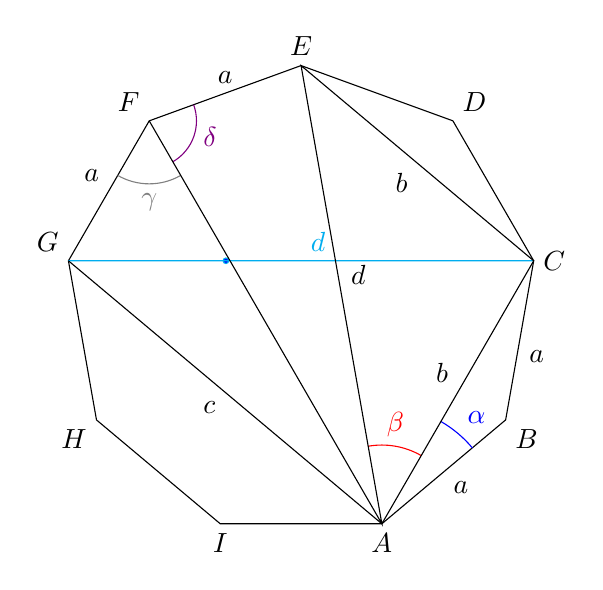
\begin{tikzpicture}
 \foreach \v in {0,...,8} {
  \pgfmathsetmacro{\sinv}{sin(40*\v+20)}
  \pgfmathsetmacro{\cosv}{-cos(40*\v+20)}
  \coordinate (V\v) at (3*\sinv,3*\cosv);
 }
%\coordinate (V9) at (V6)+(0,1)
\begin{scope}[scale=2]
 \draw (V0)node[below]{$A$}
 -- node[midway,below right]{$a$} (V1) node[below right]{$B$} 
 -- node[midway,below right]{$a$} (V2) node[right]{$C$}
 -- (V3) node[above right]{$D$} 
 -- (V4) node[above]{$E$}
 -- (V5) node[midway,above]{$a$} node[above left]{$F$}
 -- (V6) node[midway,above left]{$a$} node[above left]{$G$}
 -- (V7) node[below left]{$H$}
 -- (V8) node[below]{$I$} 
 -- cycle;
 \draw[cyan,fill=blue] (V2)
  -- node[midway,above right]{$d$} (V6)
  -- +(1,0) circle(0.5pt);
 
\pgfmathsetmacro{\ABx}{sin(50)}
\pgfmathsetmacro{\ABy}{cos(50)}
\pgfmathsetmacro{\ACx}{sin(30)}
\pgfmathsetmacro{\ACy}{cos(30)}
\draw[blue] (V0) ++(0.75*\ABx,0.75*\ABy) arc(40:60:0.75) node[midway,above right]{$\alpha$};
\draw[red] (V0) ++(0.5*\ACx,0.5*\ACy) arc (60:100:0.5) node[midway,above]{$\beta$};
\draw[violet] (V5) ++(0.3*\ACx,-0.3*\ACy) arc(300:380:0.3) node[midway,right]{$\delta$};
\draw[gray] (V5) ++(-0.4*\ACx,-0.4*\ACy) arc(240:300:0.4) node[midway,below]{$\gamma$};
  
 \draw (V0)
 -- node[midway,above left]{$b$} (V2)
 -- node[midway,below left]{$b$} (V4)
 -- node[midway,above right]{$d$} (V0)
 -- node[midway,below left]{} (V5);
 \draw (V0)
 -- node[midway,below left]{$c$} (V6);
\end{scope}
\end{tikzpicture}
\caption{The nonagon perimeter side $a$ and the three internal diagonals $b,c,d$.
Also shown the base angle $\alpha$ and three more $\beta = 2\alpha$, $\gamma=3\alpha$
and $\delta = 4\alpha$.}
\label{fig:nonagon}
\end{figure}

From figure \ref{fig:nonagon} we can can calculate $\cos\alpha$ inspecting 
isosceles $\triangle{ABC}$ ($\overline{AB} = \overline{AC} = a$):
\begin{align}
a^2 &= a^2 + b^2 - 2ab\cos\alpha \nonumber\\
b^2 &= 2ab\cos\alpha \implies \boxed{b = 2a\cos\alpha} \label{eq:cos-alpha}
\end{align}

We calculate $\cos\beta$ inspecting isosceles $\triangle{ACE}$
($\overline{AB} = \overline{AE} = b$):
\begin{align}
b^2 &= b^2 + d^2 - 2bd\cos\beta \nonumber\\
d^2 &= 2bd\cos\beta \implies \boxed{d = 2b\cos\beta} \label{eq:cos-beta}
\end{align}

We calculate $\cos\delta$ inspecting isosceles $\triangle{AEF}$
($\overline{AE} = \overline{AF}$ = d):
\begin{align}
d^2 &= a^2 + d^2 - 2ad\cos\delta \nonumber\\
a^2 &= 2ad\cos\delta \implies \boxed{ a = 2d\cos\delta } \label{eq:cos-delta}
\end{align}

From equations \ref{eq:cos-alpha}, \ref{eq:cos-beta} and \ref{eq:cos-delta} we have:
\begin{equation}\label{eq:cos-alpha-beta-delta}
\cos\left({\begin{array}{c} \alpha\\ \beta\\ \delta\\ \end{array}}\right)
= \left({\begin{array}{c}
\dfrac{b}{2a}\\[10pt]
\dfrac{d}{2b}\\[10pt]
\dfrac{a}{2d}\\[10pt]
\end{array}}\right)
\end{equation}

From equation \ref{eq:cosines-alpha-beta-delta-sum} $\cos\alpha = \cos\beta + \cos\delta$:
\begin{align}
\frac{b}{2a} &= \frac{d}{2b} + \frac{a}{2d}
 \implies \boxed{ \frac{1}{a/b} = \frac{1}{b/d} + \frac{1}{d/a}}
\end{align}

\end{document}
